\documentclass[aspectratio=169,11pt]{beamer}
\usepackage{teaching_slides}
\usepackage{listings}

\lstset{
  language=R,
  basicstyle=\ttfamily\tiny,
  backgroundcolor=\color{gray!5},
  frame=single,
  rulecolor=\color{gray!50},
  keywordstyle=\color{blue!70!black},
  commentstyle=\color{green!40!black},
  stringstyle=\color{orange!90!black},
  columns=flexible,
  keepspaces=true,
  showstringspaces=false,
  breaklines=true
}


\usepackage{inconsolata} % nice monospace font


\title{Difference in Differences}
\author{Chris Conlon}
\institute{Applied Econometrics}
\date{\today}

\begin{document}
\frame{\titlepage}




\begin{frame}{Recall: Fundamental Problem of Causal Inference}
\begin{columns}[T] % align columns
\begin{column}{.65\textwidth}
Fundamental Problem of Causal Inference
\begin{itemize}
\item We don't observe the \alert{counterfactual} $Y_i(1-D_i)$.
\item For a single individual we either observe $Y_i(1)$ \alert{or} $Y_i(0)$ but never both!
\begin{itemize}
\item ex: We don't see what your wage would have been if you didn't attend college.
\item ex: We might know your cholesterol before you took Lipitor, but we don't know what it would be today if you didn't take Lipitor.
\end{itemize}
\end{itemize}
\end{column}%
\hfill%
\begin{column}{.38\textwidth}

  \vspace{20pt}
  
  $Y_{i} = D_{i}\cdot Y_{i}(1) + (1-D_{i}) \cdot Y_{i}(0)$\\
  \vspace{20pt}
  \begin{tabular}{ccccc}
    \toprule
    i & $Y_{i}(1)$ &  $Y_{i}(0)$ & $D_{i}$ & $X_{i}$ \\
    \midrule
    1 &     1      &     \alert{?}      &   1   & 3.2 \\
    2 &     0      &     \alert{?}      &   1   & 1.7 \\
    3 &     \alert{?}      &     0      &   0   & 2.5 \\
     & &  $\vdots$ & & \\
    $n$ &     \alert{?}      &     1      &   0   & -1.5 \\    
  \end{tabular}
\end{column}%
\end{columns}
\end{frame}


\begin{frame}{How do we construct the counterfactual?}
We observe $Y_i(D_i)$ but not $Y_i(1-D_i)$, how do we estimate it?\\

\begin{description}
  \item [Event Study:] Compare $Y_{t+k}(1)$ to $Y_{t-j}(0)$ before and after an event at $t$.
  \item [Matching:] Compare $Y_i(1)$ to $Y_j(0)$ for $i \neq j$ but where $X_i = X_j$.
  \item [\alert{Difference in Difference:}] Compare $Y_{i,t}(1)-Y_{i,t-1}(0)$ to $Y_{j,t}(0)-Y_{i,t-1}(0)$  for some $j \neq i$.
  \item [Synthetic Control:] Compare $Y_{i,t}(1)-Y_{i,t-1}(0)$ to $\overline{Y}_{-i,t}(0)-\overline{Y}_{-i,t-1}(0)$ for some average over $j \neq i$ so that $X_{i,t} \approx \overline{X}_{-i,t}$.

\end{description}
\end{frame}


\section{Difference in Differences}

\begin{frame}{Motivation: Recap Matching}
Matching estimators had some advantages:
\begin{itemize}
\item Limited assumptions on \alert{functional forms}
\item We could do nearest neighbor matching and use kernels to compute treatment effects
\end{itemize}
Matching estimators had some drawbacks:
\begin{itemize}
\item Treated patients were ``matched'' to control patients based only on \alert{observable characteristics}
\begin{itemize}
\item Ignored \alert{selection on unobservables}.
\end{itemize}
\item Relied on \alert{cross sectional} variation to construct a control group.
\end{itemize}
\end{frame}


\begin{frame}{Motivation}
IV estimators resolve some of those issues but
\begin{itemize}
\item Good IV are in short supply!
\end{itemize}
 Often (in this course at least) we have access to \alert{panel data}.
\begin{itemize}
\item What if we could use panel data to control for \alert{unobserved heterogeneity} within a treated individual/group?
\end{itemize}
\alert{Difference in Difference} estimators are like the opposite of matching
\begin{itemize}
\item \alert{Strong} assumptions on \alert{functional form}
\item but... allow for \alert{unobservable heterogeneity} in outcomes.
\end{itemize}
\end{frame}


\section{Intro to Difference in Difference}


\begin{frame}{Differences}
\begin{itemize}
  \item Consider using OLS to estimate
  \begin{align*}
  Y_{i}=\beta_{0}+\beta_{1}\cdot D_{i}+ \varepsilon_{i}
  \end{align*}
  when $D_i \in \left\{ 0,1\right\}$ is assigned randomly.

  \medskip
  \item From the OLS formula and a little algebra, we can show that
  \begin{align*}
  \hat{b}_1 = \bar{Y}_{1} - \bar{Y}_{0}
  \end{align*}
  where $\bar{Y}_{1}$ is the sample mean of $Y_i$ conditional on
  $D_i = 1$, and similarly $\bar{Y}_{1}$ is the sample mean conditional on $D_i = 0$.

  \medskip
  \item Note: this loops us back to the treatment effects setup, where
  we were comparing conditional means.

\end{itemize}
\end{frame}



\begin{frame}{Differences-in-Differences I}
\begin{itemize}
  \item {\bf Differences-in-differences} is a {\bf quasi-experimental} design
  that attempts to deal with selection by focusing how treatment and control
  groups change between two periods

  \smallskip
  \item Consider the model  
  \begin{align*}
  Y_{it}=\beta_{0}+\beta_{1} \cdot D_{it}+\boldsymbol{\beta}_2' {\bf X}_{i}+ \beta_{post}  Post_t  + \varepsilon_{it},
  \end{align*}
  and furthermore suppose that
  \begin{itemize}
    \item Some variables in ${\bf X}$ may be unobserved
    \item $D_{it}$ is not random and may be correlated with ${\bf X}_{i}$
    \item $Post_t$ is a dummy variable for the post-treatment period $t=2$
    \item Each individual $i$ is observed (at least) twice
    \item For some individuals, $D_{it}$ changes over time ({\bf natural experiment})
    \item ${\bf X}_{i}$ does not change over time
  \end{itemize}

\end{itemize}
\end{frame}


\begin{frame}{Differences-in-Differences II}
\begin{align*}
  Y_{it}=\beta_{0}+\beta_{1}\cdot D_{it}+\boldsymbol{\beta}_2' {\bf X}_{i} + \beta_{post}  Post_t  + \varepsilon_{it},
\end{align*}

\begin{itemize}
  \item Let $\Delta Y_{i}$ represent the change in $Y_{it}$ between two time periods:
  \begin{align*}
  \Delta Y_{i} = Y_{i2} - Y_{i1},
  \end{align*}
  and define $\Delta D_i$ and $\Delta \varepsilon_i$ similarly.

  \medskip
  \item A differenced regression equation:
  \begin{align*}
  \Delta Y_{i}=\beta_{post} + \beta_{1} \Delta D_{i}+ \Delta \varepsilon_{i}
  \end{align*}

\end{itemize}
\end{frame}


\begin{frame}{Differences-in-Differences III}
\begin{align*}
  \Delta Y_{i}=\beta_{post} + \beta_{1}  \cdot \Delta D_{i}+ \Delta \varepsilon_{i}
\end{align*}

\begin{itemize}
  \item Applying OLS to the differenced regression equation will provide unbiased
  estimates as long as
  \begin{align*}
  \E\left[ \Delta \varepsilon_{i} \mid \Delta D_{i} \right] =0.
  \end{align*}
  Exogeneity assumptions of this form are known as the {\bf parallel trends
  assumption}.

\end{itemize}
\end{frame}

\begin{frame}{Differences-in-Differences IV}
\begin{align*}
  \Delta Y_{i}=\beta_{post} + \beta_{1} \cdot \Delta D_{i}+ \Delta \varepsilon_{i}
\end{align*}
\begin{itemize}
  \item From before, recall that the OLS estimator for a simple experiment
  amounted to the difference in conditional means of the outcome variable.

  \medskip
  \item The same is true here, but now we start with an outcome variable that
  is differenced over time. Suppose that for some observations, $\Delta D_{i}=1$
  (treatment group), and for others $D_{i1}=D_{i2}=0$ (untreated group).
  \begin{align*}
\hat{b}_{1,DID}=\overline{\Delta Y}_{T}-\overline{\Delta Y}_{C}
\end{align*}
where $\overline{\Delta Y}_{T}$ is the conditional mean of $\Delta Y_{i}$
for the treatment group, and $\overline{\Delta Y}_{C}$ is the conditional
mean of $\Delta Y_{i}$ for the control group.

\end{itemize}
\end{frame}


\begin{frame}{The Appeal of DID}
\begin{itemize}
  \item The DID strategy is robust to a form of selection bias
  (when, the selection is related to persistent characteristics).
  Simple differences across treatment and control groups would not be.

  \medskip
  \item DID estimates are also robust to aggregate shocks or time effects. Simple differences
  over time for the treatment group would not be.

  \medskip
  \item DID can be used to study many ``natural experiments,'' where something
  changes for one group but not for an otherwise similar group.

\end{itemize}
\end{frame}

\section{A Famous Example: Card and Krueger (AER 1994)}

\begin{frame}{A Famous Example: Card and Krueger (AER 1994)}
\begin{itemize}
\item On April 1, 1992 NJ raises its minimum wage from $\$4.25\rightarrow \$5.05$ per hour.
\item Question: Econ 101 predicts this will \alert{reduce demand for low wage workers}
\begin{itemize}
\item Focus on fast food restaurants (since they pay min wage)
\item Focus on starting wage (avoid tenure, high turnover)
\end{itemize}
\item Survey 410 restaurants in NJ (treated group) and eastern PA (control group).
\item Idea: Compare \alert{change} in wages in $NJ$ to $PA$:  $\Delta_{DD} = \Delta_{NJ}- \Delta_{PA}$
\begin{itemize}
\item Wave 1: February 15-March 4, 1992
\item Wave 2: November 5 - December 31, 1992
\end{itemize}
\end{itemize}
\end{frame}

\begin{frame}{Balance Table: Covariates}
\begin{center}
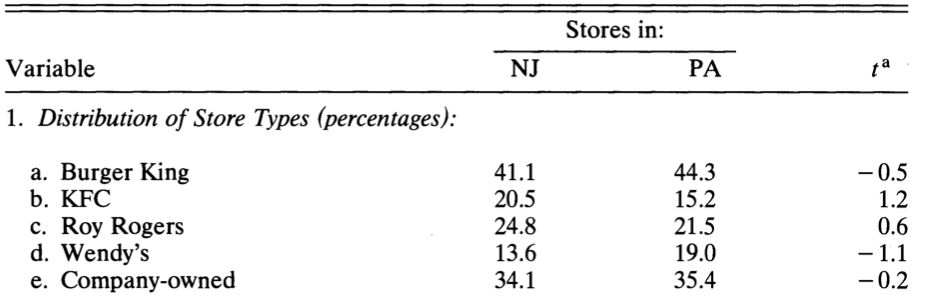
\includegraphics[width=2.25in]{./resources/ck_tab2b.png}\\
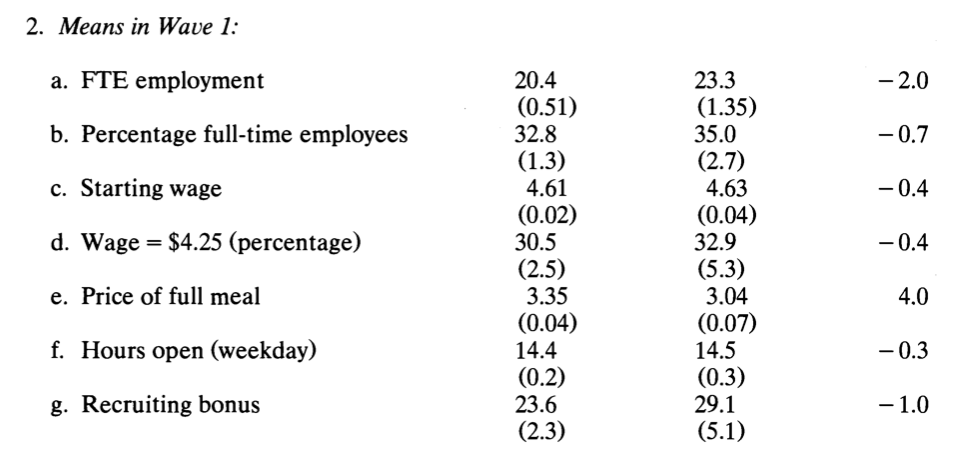
\includegraphics[width=2.25in]{./resources/ck_tab2c.png}\\
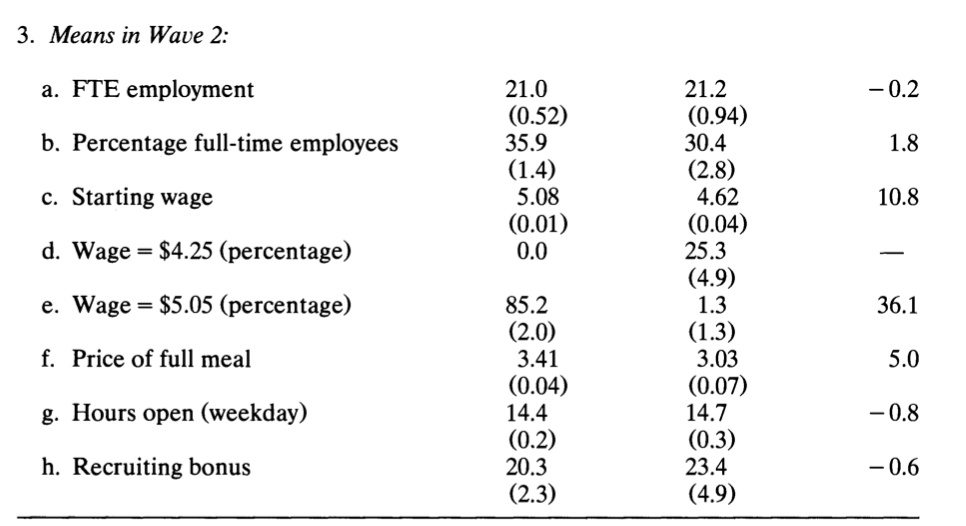
\includegraphics[width=2.25in]{./resources/ck_tab2a.png}
\end{center}
\end{frame}



\begin{frame}{Distribution of Wages}
\begin{center}
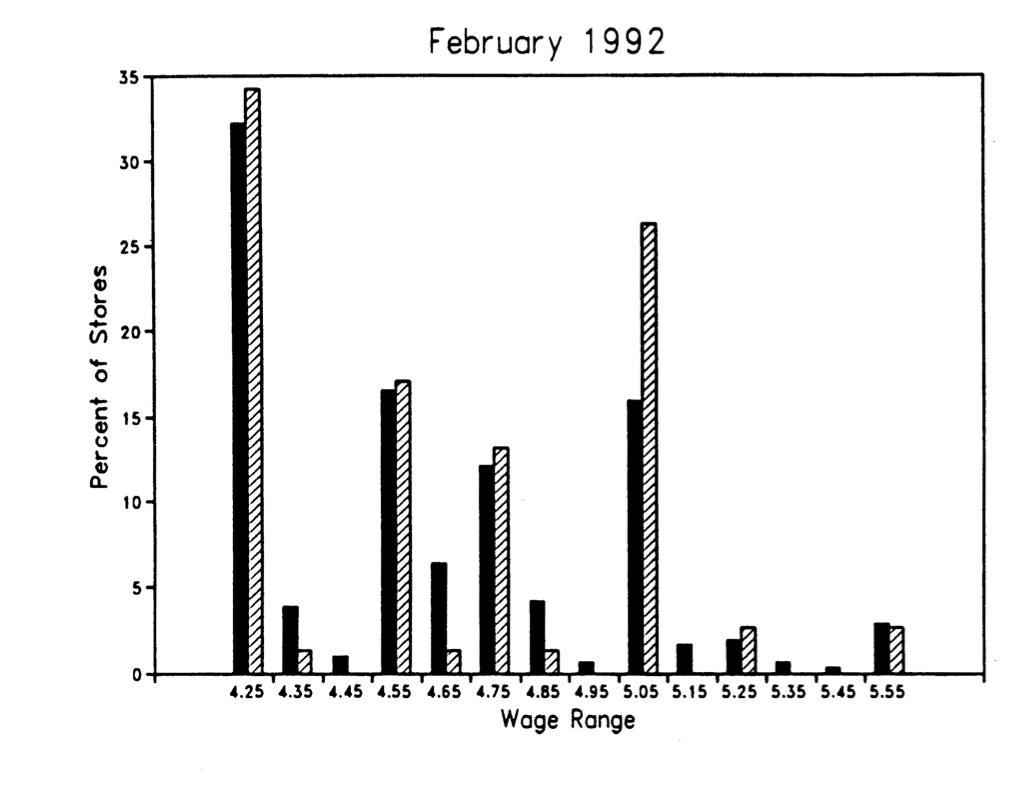
\includegraphics[width=2.75in]{./resources/ck_fig1b.png}
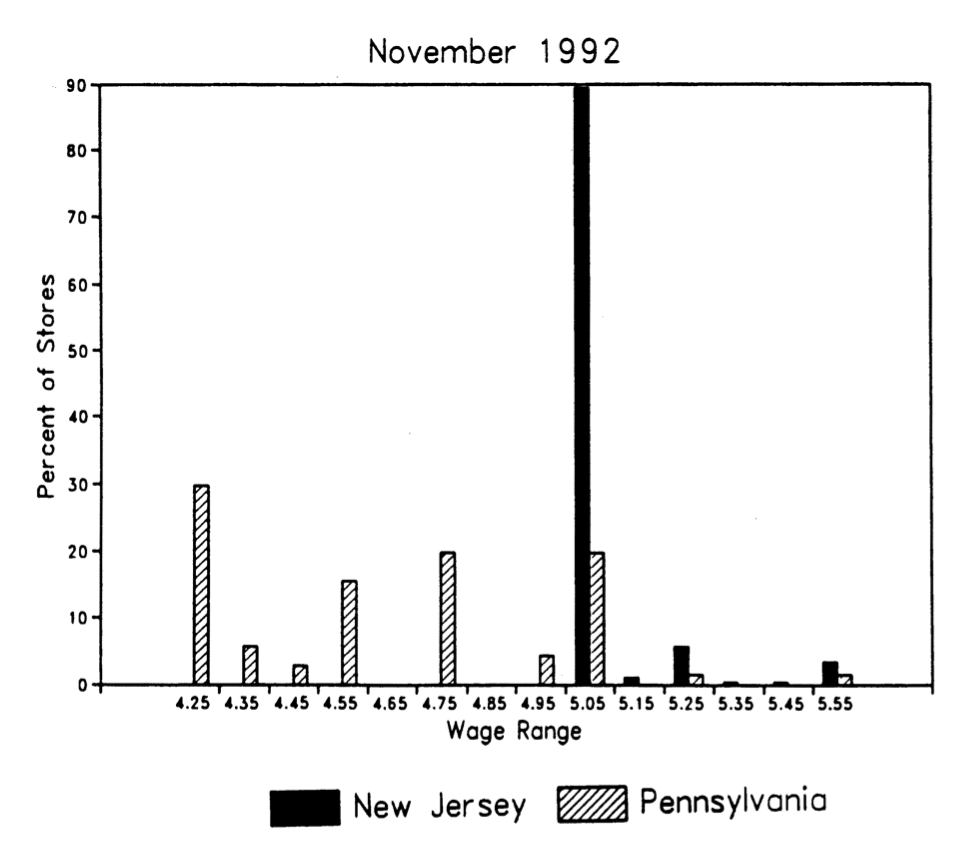
\includegraphics[width=2.5in]{./resources/ck_fig1a.png}
\end{center}
\end{frame}


\begin{frame}{Differences in Wages : 2 x 2 Table}
\begin{center}
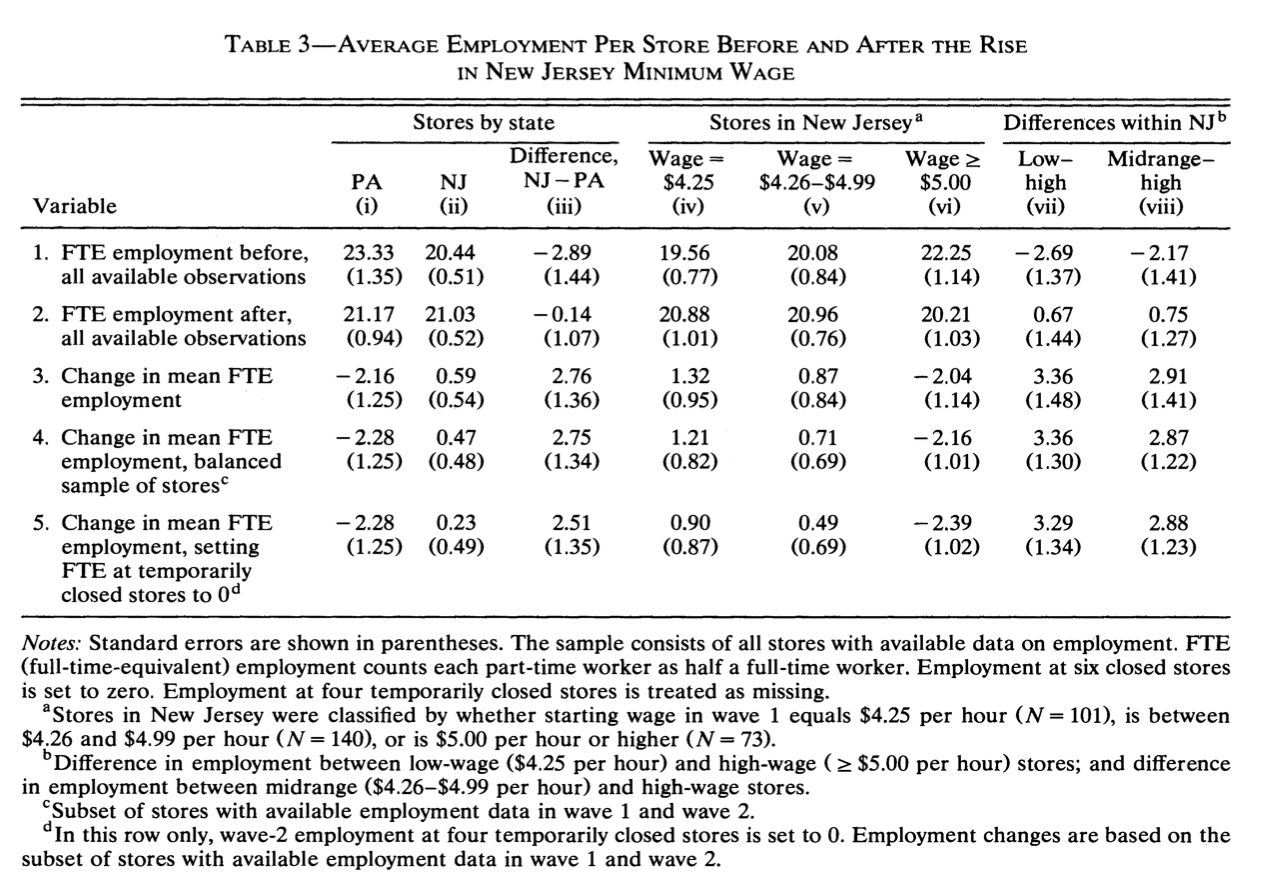
\includegraphics[width=4.25in]{./resources/ck_tab3.png}
\end{center}
\end{frame}

\begin{frame}{Outcome Equation}
\begin{itemize}
\item Differences lack any covariates (different fast food chains).
\item Also $\Delta_{PA}<0$ and $\Delta_{NJ} > 0$ (!)
\item Recall $i$ denotes stores, $t \in {1,2}$. Run the following regression:
\begin{align*}
Y_{it}&=\beta X_{it} +\alpha \cdot [i \in \text{NJ}] +  \gamma \cdot \text{After}_{t}  + \delta \cdot NJ_i \times After_{t} +u_{i}\\
Y_{it}&=\beta X_{it} +\alpha \cdot [\text{wage gap}_{i}] +  \gamma \cdot \text{After}_{t}  + \delta \cdot \text{wage gap}_{i} \times After_{t} +u_{i}
\end{align*}
\item $\alpha$ is mean difference between $NJ$ and $PA$
\item $\gamma$ is mean difference between period $1$ and $2$
\item $\delta$ is the parameter of interest, the \alert{difference in difference}
\item $\text{wage gap}_{i} = [\text{min wage}_{i,2}-w_{i1} ]_{+} =\max\{0, \text{min wage}_{i,2}-w_{i1}\} $.\\
 (How much do you need to raise $t=1$ wages to achieve minimum wage in $t=2$?)
\end{itemize}
\end{frame}

\begin{frame}{Differences in Wages}
\begin{center}
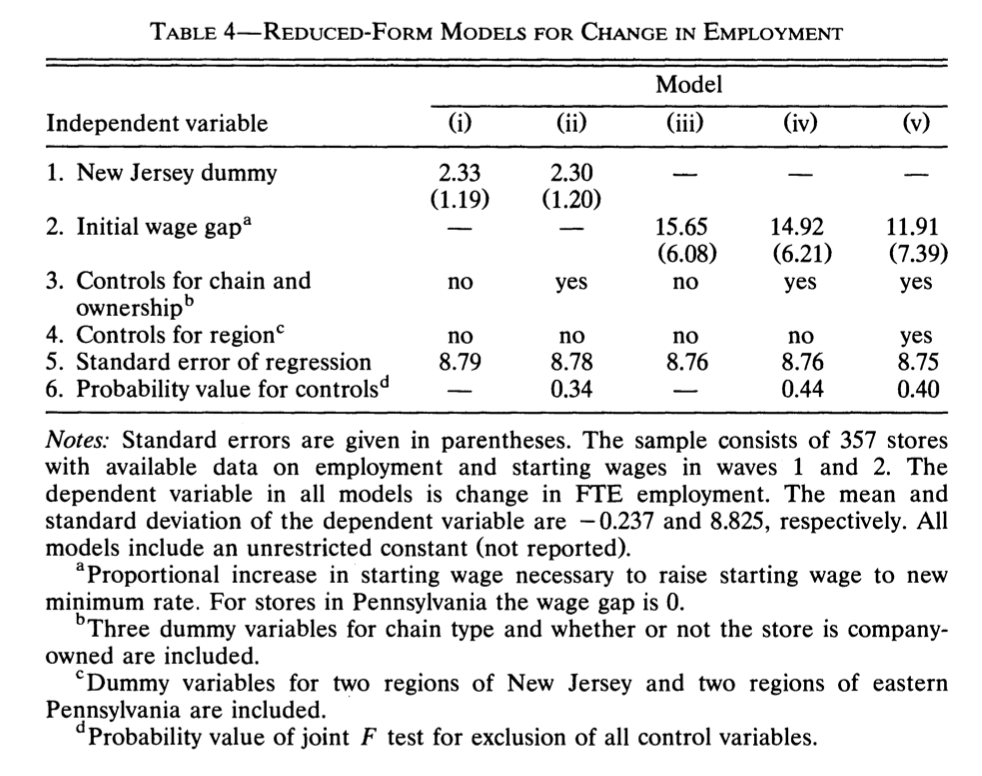
\includegraphics[width=4in]{./resources/ck_tab4.png}
\end{center}
\end{frame}


\begin{frame}{Parallel trends vs pre-trends}
\begin{itemize}
  \item When the data is available, researchers typically check {\bf pre-trends}
  as a way of motivating the parallel trends assumption.
  \begin{itemize}
    \item That is, look at how the control and treatment groups evolve in several
    periods preceding the time of treatment to see if they were changing in similar
    ways over time.
  \end{itemize}
  
  \smallskip
  \item This is a worthwhile check, and we should certainly worry about the plausibility
  of the parallel trends assumption if the pre-trends are not parallel.
  
  \smallskip
  \item However, the parallel trends assumption is about what \emph{would have happened}
  immediately at the time of treatment in the absence of treatment, not about what
  happened before treatment. Thus, establishing parallel pre-trends {\bf does not} establish
  the parallel trends assumption.
  \begin{itemize}
  \item  Just as we can't test exogeneity within the OLS framework, we can't test
  the parallel trends assumption within the DiD framework. 
  \end{itemize}
\end{itemize}
\end{frame}

\begin{frame}{Parallel trends vs pre-trends: example}
Consider the NJ minimum wage study. Here's a concern that would not be assuaged by seeing parallel pre-trends:
\begin{itemize}
  \item  If the minimum wage changed 
  because a new administration was elected in NJ and they implemented a portfolio
  of new policies, then the minimum wage change might have been just one of several
  ways in which NJ and PA were diverging at the time.  
  
  \smallskip
  \item Some of the other policy changes might have led to greater labor force participation and/or
  incentivized businesses to hire more.
  
  \smallskip 
  \item Because of these other changes, we would expect NJ's restaurant employment to move
  differently from PA's in 1992 even if the minimum wage change had not happened.

  \smallskip
  \item This could all be true even if NJ and PA were evolving similarly before 1992. The point is that
    the treatment was one thing that diverged in 1992, and if one thing was diverging at that point,
    perhaps other things were also diverging. 
\end{itemize}
\end{frame}




\begin{frame}{DID Experiments}
\begin{itemize}
  \item Recall that before we argued that experimental
  effects can be estimated with regressions using additional
  covariates (controls) even though they don't need to be.

  \medskip
  \item Similarly, they can be estimated using differences-in-differences
  rather than simple differences. They don't need to be, as with
  randomized treatment, the treatment and control groups should have
  similar baselines.

\end{itemize}
\end{frame}

\begin{frame}{NJ Minimum Wage Follow-Up}
\begin{itemize}
  \item The study has been controversial, and it has had a
  big impact on policy discussions.

  \medskip
  \item Card and Krueger update their conclusion
  in a 2000 follow up:
  \begin{quotation}
The increase in New Jersey's minimum wage probably
had no effect on total employment in New Jersey's
fast-food industry, and possibly had a small positive
effect.
  \end{quotation}

  \smallskip
  \item There have been \emph{many} criticisms of the paper,
  including studies showing that the result is not robust to the
  sample of stores and data source used, and concerns about
  the external validity of the focus on only fast food stores.

  \smallskip
  \item Also see studies based on Seattle's 2015 minimum wage change. 
\end{itemize}
\end{frame}



\section{A More General Method}



\begin{frame}{Difference in Difference: General Approach}
\begin{align*}
\text{Potential outcome in period } 1&=Y_{i 1}(0)\\
\text{Potential outcome in period } 2&=\left\{ \begin{array}{ll}
Y_{i 2}(1) & \text { if } D_{i 2}=1 \\ 
Y_{i 2}(0) & \text { if } D_{i 2}=0
\end{array}\right\}\\
\end{align*}
\begin{center}
\begin{tabular}{|c|c|c|}
\hline & Treatment & Control \\
\hline Before & $Y_{i 1}(0)$ & $Y_{i 1}(0)$ \\
After & $Y_{i 2}(1)$ & $Y_{i 2}(0)$ \\
\hline
\end{tabular}
\end{center}
We can write the outcome as:
\begin{align*}
Y_{i t}=D_{i t} \cdot Y_{i t}(1)+\left(1-D_{i t}\right) \cdot Y_{i t}(0)=D_{i t} \cdot\left(Y_{i t}(1)-Y_{i t}(0) \right)+Y_{i t}(0)
\end{align*}
\end{frame}

\begin{frame}{Difference in Difference: General Approach}
\small
Consider the first difference $\Delta Y_{it} = Y_{i2} - Y_{i1}$:
\begin{align*}
\Delta Y_{it}  = D_{i2} \cdot \left(Y_{i2}(1) - Y_{i2}(0) \right) +  Y_{i2}(0) - Y_{i1}(0)
\end{align*}
For treated group (first difference):
\begin{align*}
\E[\Delta Y_{it} \mid D_{i2}=1]  = \overbrace{\E\left[Y_{i2}(1) - Y_{i2}(0) \mid T_{i2}=1 \right]}^{\alert{ATT}} +  \overbrace{\E\left[Y_{i2}(0) - Y_{i1}(0) \mid D_{i2}=1 \right]}^{\alert{\gamma(1)}}
\end{align*}
For control group (second difference):
\begin{align*}
\E[\Delta Y_{it} \mid D_{i2}=0]  = \overbrace{\E\left[Y_{i2}(0) - Y_{i1}(0) \mid D_{i2}=0 \right]}^{\alert{\gamma(0)}}
\end{align*}
The DiD (difference in difference) estimator
\begin{align*}
\Delta_{DD} = \E[\Delta Y_{it} \mid D_{i2}=1]  - \E[\Delta Y_{it} \mid D_{i2}=0]  
\end{align*}
\end{frame}



\begin{frame}{Difference in Difference: Parallel Trends}
\small
\begin{itemize}
\item If $\gamma(1) = \gamma(0)$ then the DiD estimator cancels and we are left with the $\Delta_{DD} = \text{ATT}$.
\item This is the \alert{parallel trends assumption}
\begin{align*}
\E\left[Y_{i2}(0) - Y_{i1}(0) \mid D_{i2}=0 \right] = \E\left[Y_{i2}(0) - Y_{i1}(0) \mid D_{i2}=1 \right]
\end{align*}
\item Absent the treatment effect, both treatment and control would evolve identically over time.
\item But, treatment and control groups can start from very different places...
\begin{align*}
\E\left[Y_{i t}(0) \mid D_{i 2}=1\right] \neq E\left[Y_{i t}(0) \mid D_{i 2}=0\right], t=1,2
\end{align*}
\item And have selection on treatment effects...
\begin{align*}
\E\left[Y_{i 2}(1)-Y_{i 2}(0) \mid D_{i 2}=1\right] \neq \E\left[Y_{i 2}(1)-Y_{i 2}(0) \mid D_{i 2}=0\right]
\end{align*}
\end{itemize}
\end{frame}


\begin{frame}{Parallel Trends}
\begin{figure}
\centering
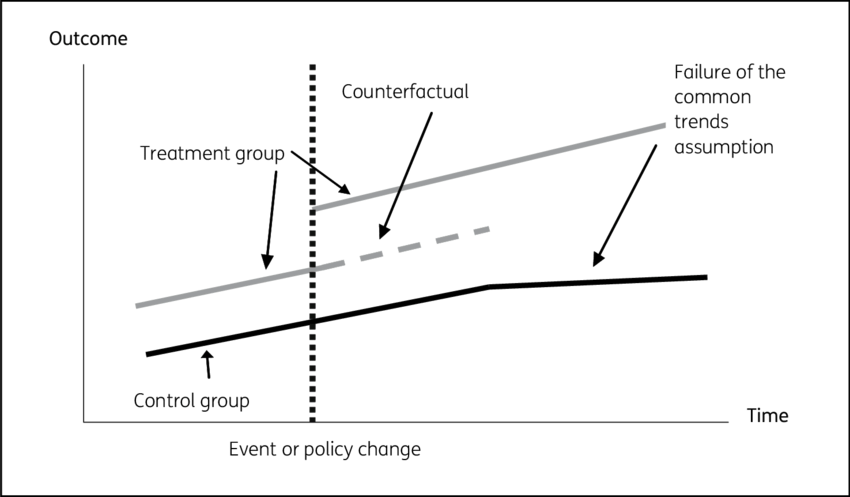
\includegraphics[width=5in]{./resources/common_trend.png}
\end{figure}
\end{frame}



\begin{frame}{Difference in Differences: Limitations}
\begin{enumerate}
\item Functional form restrictions
\begin{itemize}
\item \alert{Parallel trends} assumes that absent treatment that we add $\gamma_2 - \gamma_1$ to each unit
\item Because this is \alert{additive} it is not invariant to transformations $f(Y_{it})$ (ie: taking logs)
\end{itemize}
\item Parallel Trend Assumption is \alert{not testable}
\begin{itemize}
\item Best we can hope is that it looks similar in the pre-period
\end{itemize}
\item Compositional Effects: the treatment may affect who is in each group
\begin{itemize}
\item Restaurants could close in NJ and open nearby in PA to avoid minimum wage.
\item A good job training program may lead to migration, etc.
\item One approach: redefine the population so that it doesn't endogenously respond to treatment
\begin{itemize}
\item Recover something, but probably not ATT anymore...
\end{itemize}

\end{itemize}

\end{enumerate}

\end{frame}

\begin{frame}{Checking Pre-Trend: Card Krueger (2000)}
\begin{figure}
\centering
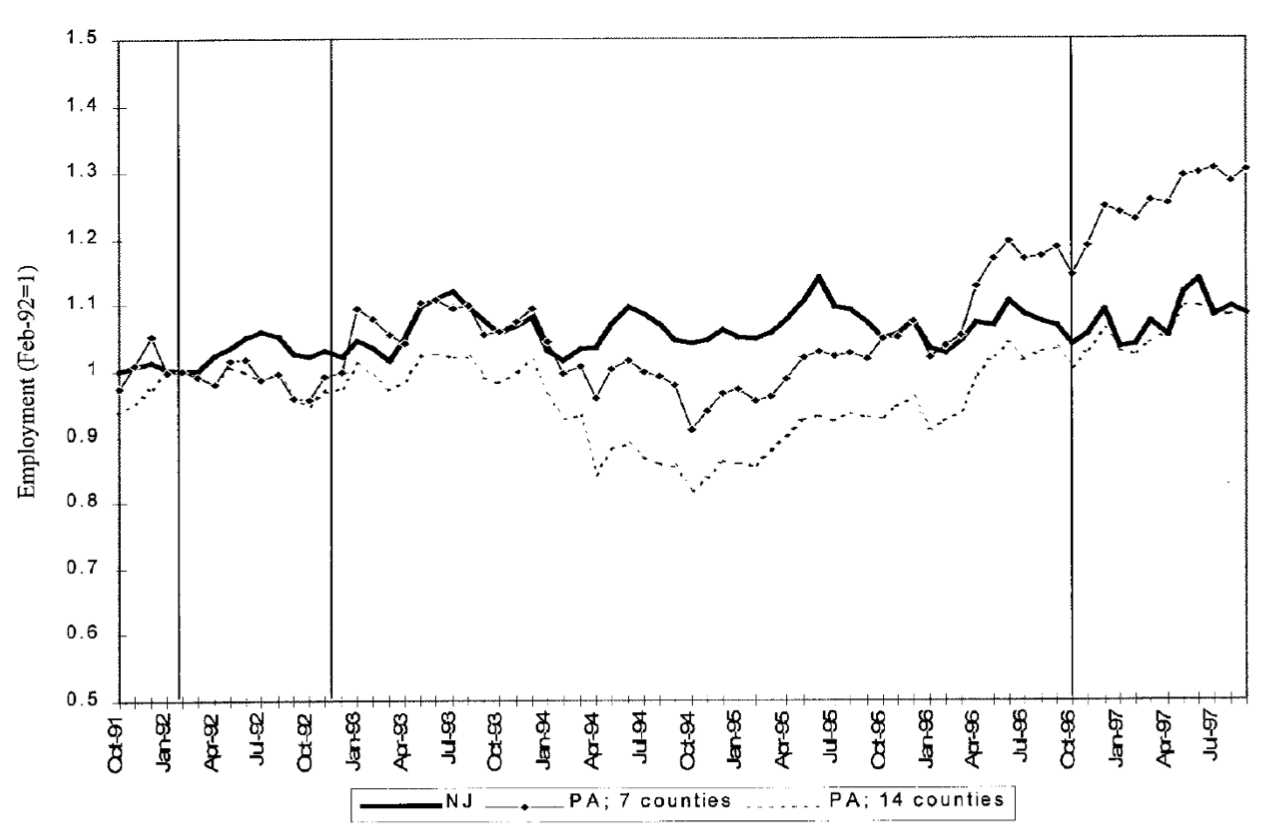
\includegraphics[width=4.5in]{./resources/card_krueger_2000.png}
\end{figure}
\end{frame}



\begin{frame}{Difference in Differences}
Just like in Card and Kruger, we can write as a regression equation:
\begin{align*}
 Y_{it} =\alpha_i +\gamma_t +\beta X_{it} + \delta_i D_{it}  + u_{it}
 \end{align*}
\begin{itemize}
\item Suppose we wish to evaluate a training program for those with low
earnings. Let the threshold for eligibility be $B$.
\item We have a panel of individuals and those with low earnings qualify for
training, forming the treatment group.
\item Those with higher earnings form the control group. 
\item Now the low earning group is low for two reasons
\begin{enumerate}
\item They have low permanent earnings ($\alpha_i$ is low) - this is accounted for by diff in diffs.
\item They have a negative transitory shock ($u_{i1}$ is low) - this is not accounted for by diff in diffs.
\end{enumerate} 
\end{itemize}
\end{frame} 

\begin{frame}{The ``Ashenfelter Dip'' (Heckman and Smith 2000)}
\begin{figure}
\centering
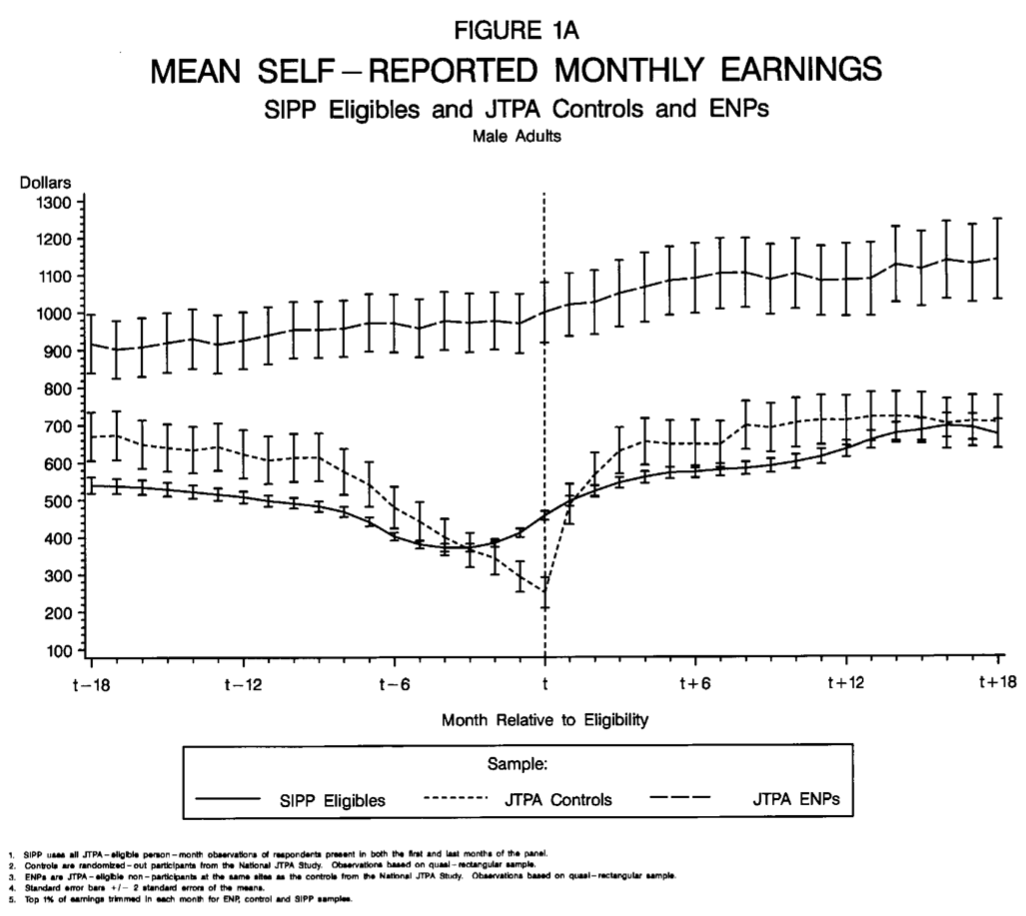
\includegraphics[width=4.25in]{./resources/ashenfelter_dip.png}
\end{figure}
\end{frame}

\begin{frame}{Difference in Differences}
\small
\begin{itemize}
\item  \#2 above violates the assumption {\small $\E[Y_{i2}(0) - Y_{i1}(0) \mid D] = \E[Y_{i2}(0) - Y_{i1}(0)]$}. 
\item To see why note that those participating into the program are such
that {\small $Y_{i0}(0) < B$}. Assume for simplicity that the shocks {\small $u$} are {\small $iid$}. Hence {\small $u_{i1} < B- \alpha_i - \gamma_1$}. 
This implies: 
{\small $$\E[Y_{i2}(0)- Y_{i1}(0) \mid D=1] = \gamma_2 = \gamma_1 - \E[u_{i1} \mid u_{i1} <  B-\alpha_i - \gamma_1]$$}
For the control group:
{\small $$\E[Y_{i2}(0) - Y_{i1}(0) \mid D=1] = \gamma_2 = \gamma_1 - \E[u_{i1} \mid u_{i1} >  B-\alpha_i - \gamma_1]$$}
So that:
\begin{align*}
& \E[Y_{i2}(0) - Y_{i1}(0) \mid D=1] - \E[Y_{i2}(0) - Y_{i1}(0) \mid D=0] =\\
&  \E[u_{i1} \mid u_{i1} >  B-\alpha_i - \gamma_1] - \E[u_{i1} \mid u_{i1} < B-\alpha_i - \gamma_1]  >0
  \end{align*}
 \item This is effectively regression to the mean: those unlucky enough to have a bad shock recover and show greater growth relative to those with a good shock. The nature of the bias depends on the stochastic properties of the shocks and how individuals select into training.
\end{itemize}
\end{frame} 

% \begin{frame}{Difference in Differences}
% Ashefelter (1978) was one of the first to consider difference in differences to evaluate training programs.
% 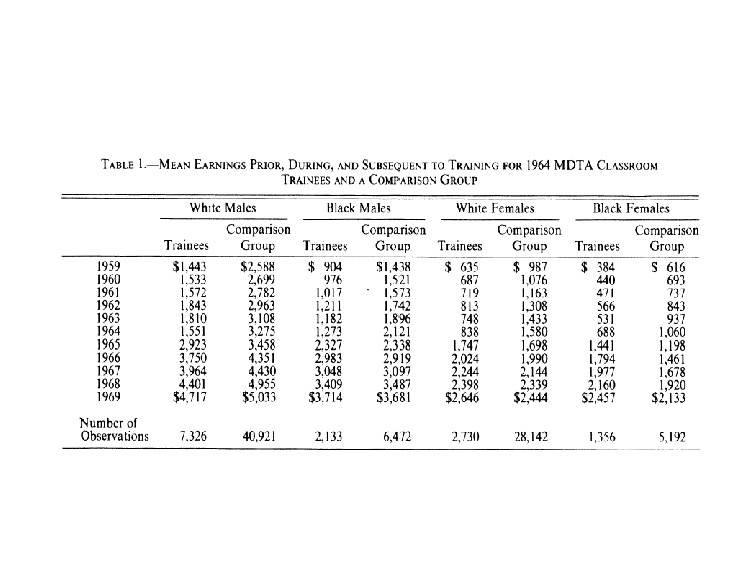
\includegraphics[scale=1]{./resources/ashefelter1.pdf}
% \end{frame}

% \begin{frame}{Difference in Differences}
% Ashenfelter (1978) reports the following results.
% \begin{figure}
% \centering
% 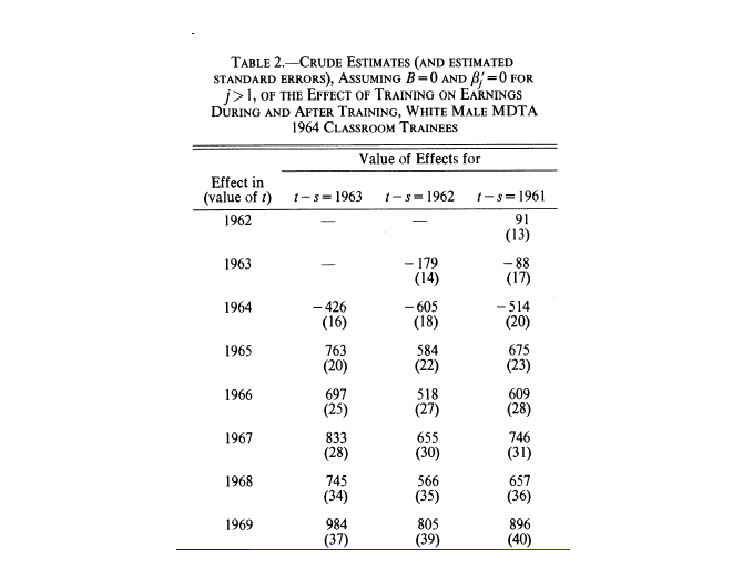
\includegraphics[scale=.85]{./resources/ashefelter2.pdf}
% \end{figure}
% \end{frame}

\begin{frame}{Difference in Differences}
\begin{itemize}
\item The assumption on growth of the non-treatment outcome being independent of assignment to treatment may be violated, but it may still be true conditional on $X$.
\item Consider the assumption
\begin{align*}
\E[Y_{i2}(0)- Y_{i1}(0) \mid X,D] = \E[Y_{i2}(0)- Y_{i1}(0) \mid X]
\end{align*}
\item This is just matching assumption on a redefined variable, namely the growth in the outcomes. In its simplest form the approach is implemented by running the regression
\begin{align*}
Y_{it} = \alpha_i + \gamma_t + \delta_i D_{it} + \beta_t' X_i + u_{it}
\end{align*}
which allows for differential trends in the non-treatment growth depending on $X_i$. More generally one can implement propensity score matching on the growth of outcome variable when panel data is available.
\end{itemize}
\end{frame}

\section{Variants}

\begin{frame}{Difference in Difference in Difference}
The triple difference is also a thing:
\begin{itemize}
\item Suppose that we have: before/after, treated-state/untreated-state, treated-group (men)/ untreated-group women.
\item We can compute two D-i-D here: $\Delta_{DDD} = \Delta_{DD,state} - \Delta_{DD,gender}$ 
\item Literally difference, the difference in differences estimators.
\item As a regression: interpret the triple-interaction term (make sure to control for ALL double interactions).
\end{itemize}
\end{frame}




\begin{frame}{DID with Time-Varying Covariates}
\begin{itemize}
  \item Suppose individuals have time-varying observable covariates:
  \begin{align*}
  Y_{it}=\beta_{0}+\beta_{1}\cdot D_{it}+\boldsymbol{\beta}_2' {\bf X}_{it} + \varepsilon_{it},
  \end{align*}

  \item We can still estimate $\beta_{1}$ with a differenced linear regression,
  \begin{align*}
  \Delta Y_{i}=\beta_{1} \cdot \Delta D_{i}+\boldsymbol{\beta}_2' \Delta {\bf X}_{it} + \Delta \varepsilon_{i}
  \end{align*}
  noting that the exogeneity assumption becomes
  \begin{align*}
\E\left[\Delta\varepsilon_{i}\left|\left(\begin{array}{c}
\Delta D_{i}\\
\Delta\mathbf{X}_{i}
\end{array}\right)\right.\right]=0
\end{align*}

  \item The estimate of $\beta_{1}$ here does not correspond to a simple
  difference in differences,
  but people still describe this sort of estimation strategy as DID.
  Given Frisch-Waugh, it's still DID after controlling for ${\bf X}$.


\end{itemize}
\end{frame}

\begin{frame}{Staggered DID}
\begin{itemize}
  \item A {\bf staggered diff-in-diff} involves different groups being
    treated at different points in time. Typically, these models are
    estimated with a linear regression with two-way fixed effects. (More
    on this when we get to panel data.) 

  \medskip
  \item See \href{https://www.sciencedirect.com/science/article/pii/S0304407620303948}{Callaway and Sant'Anna}, 
    \href{https://academic.oup.com/ectj/article/26/3/C1/6604378}{de Chaisemartin and D'Haultfoeuille (2023)}
    on why this is not a valid strategy in the presence of heterogeneous
    treatment effects and for alternative estimators. (More on this in Econometrics II)

\end{itemize}
\end{frame}




\end{document}